\documentclass[comsoc,conference]{IEEEtran}
\IEEEoverridecommandlockouts
\usepackage{cite}
\usepackage{url}
\usepackage{amsmath,amssymb,amsfonts}
\usepackage{algorithmic}
\usepackage{graphicx}
\usepackage{natbib}
\usepackage{textcomp}
\usepackage{xcolor}
\usepackage{tabularx,booktabs}
\usepackage{caption}
\usepackage{subfig}
\captionsetup[table]{name=Table, labelfont=bf, labelsep=period, font=small}
\captionsetup[figure]{name=Figure, labelfont=bf, labelsep=period, font=small}
\newcolumntype{C}{>{\centering\arraybackslash}X}
\setlength{\extrarowheight}{1pt}
\def\BibTeX{{\rm B\kern-.05em{\sc i\kern-.025em b}\kern-.08em
    T\kern-.1667em\lower.7ex\hbox{E}\kern-.125emX}}
\begin{document}

\title{Aspect-based Sentiment Analysis
	\\ \large{Track: T1-02 (A Hierarchical Model of Reviews for Aspect-based Sentiment Analysis)
	\\ Team: Naive Baes}
}

\author{
	\IEEEauthorblockN{Ijaz, Ramsha}
	\IEEEauthorblockA{ramsha.ijaz@mail.mcgill.ca}
	260665762
	\and
	\IEEEauthorblockN{Rahman, Aanika}
	\IEEEauthorblockA{aanika.rahman@mail.mcgill.ca}
	260662187
	\and
	\IEEEauthorblockN{Seol, Yunheum}
	\IEEEauthorblockA{yunheum.seol@mail.mcgill.ca}
	260677676
}

\maketitle

\section{Introduction}

Sentiment analysis has been the technique used to mine opinions from customer reviews. The classical approach to this was to treat an entire sentence as a document and extract sentiments ("positive", "neutral", and "negative") based on the all words. However, it has apparent limits for sentences that contain more than one aspect with conflicting sentiments. An example for this would be a review for a restaurant that says, "The food was tasty, but I don't think it came at a reasonable price". The sentence contains two aspects (the one on quality of food and another on the price of the menu), and two contradicting sentiments. Aspect-based sentiment analysis (ABSA) addresses this issue by classifying sentiments for a given aspect label. In this approach, the previous example would have two different sentiments for both aspects would be correctly reflected.

ABSA has its own issue that it analyzes each sentence in a review independently, not taking into account the argumentative structure of the review. The paper implemented two hierarchical models (RNN, LSTM) to address this problem. These baselines were further improvised into a bidirectional LSTM that yielded better accuracy than the aforementioned models. In our paper we explore simple baselines such as the SVM and explore its accuracy with the English dataset against the baselines used by the paper. We have also implemented reproduced their baseline i.e. LSTM in the same manner as proposed in the paper. Both of the models are compared and analyzed in terms of their accuracy measure.

We are tasked with recreating the baselines reported in the paper "A Hierarchical Model of Reviews for Aspect-based Sentiment Analysis" \cite{T1-P2}. The paper considers datasets of customer reviews in 5 domains and 8 languages, with a total of 11 domain-language datasets. Given the time frame and our objective, focus will be placed on only the English datasets, which consist of two domains, restuarants (REST) and laptops (LAPT). 

\subsection{Hypotheses}

Classical machine learning algorithms fail to model long-term dependencies of words in a sequence, which are better addressed by LSTMs. Nevertheless, we expect that with appropriate representation and hyperparameter tuning, simple models can yield better results than the results of the baseline (i.e. LSTM) in the paper. Among such models, we anticipate Logistic Regression and Support Vector Machine (SVM) to be the strongest candidates. After reproducing the baseline in the paper, the LSTM can be further improved by adding deep layers. 

\section{Preprocessing}

\subsection{Data Analysis}

% no. polarities, no. reviews, no. sentences, no. sentence-aspect pairs (recall size of dataset can influence what models are best)
Each sentence in each dataset has zero to multiple associated aspects, where each aspect is composed of an entity and attribute (e.g. \texttt{FOOD\#QUALITY}), and is assigned one of three polarities (i.e. positive, neutral, negative) to describe sentiment. While there are 400-550 reviews and 2200-2600 unique sentences per dataset, following the paper, sentences with two aspects are made to occur twice, once with each aspect and sentences with no aspects to be ignored. This results in 3432 and 3774 sentence-aspect pairs as data samples for the REST and LAPT datasets respectively.

% no. categories/aspects (no. entities, no. attributes), distribution of sentences among aspects (influence threshold for aspects tested)
There are 12 and 88 potential aspect categories for REST and LAPT datasets respectively. Since the LAPT dataset has an overwhelming number of aspect categories, a threshold was set when encoding aspects such that aspects with a lower frequency are categorized under "miscellaneous", resulting in 12-15 encoded aspects per dataset.

% distribution of sentences among polarities, distribution of sentences w/ one aspect, w/ many aspects w/ same polarity, w/ many aspects w/ different polarities
As shown by the distribution of sentence-aspect pairs among polarities in Figure~\ref{fig:1}, the majority have a positive polarity and there are not many samples with a neutral polarity. Furthermore, only 10-15\% of sentences have associated aspects with differing polarities, as noted in Figure~\ref{fig:1}. Given that almost 90\% of our data have consistent polarities despite aspect, predicting polarity despite aspect per sentence may not result in poor results. 

\begin{figure}[!htbp]
    \centering
  \subfloat[\label{1a}]{%
       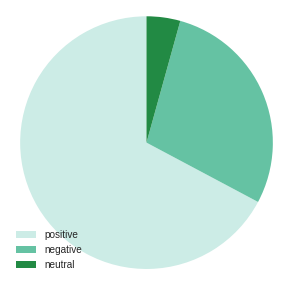
\includegraphics[width=0.45\linewidth]{images/anal_pol_REST.png}}
    \hfill
  \subfloat[\label{1b}]{%
        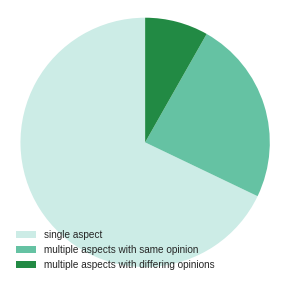
\includegraphics[width=0.45\linewidth]{images/anal_asp-pol_REST.png}}
    \\
  \subfloat[\label{1c}]{%
        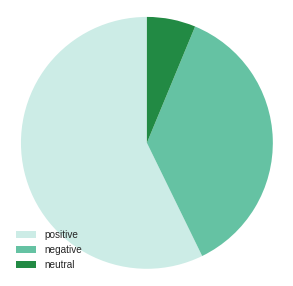
\includegraphics[width=0.45\linewidth]{images/anal_pol_LAPT.png}}
    \hfill
  \subfloat[\label{1d}]{%
        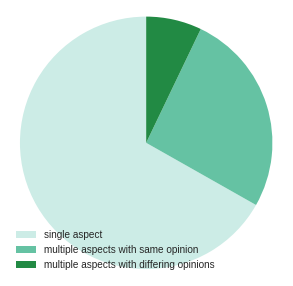
\includegraphics[width=0.45\linewidth]{images/anal_asp-pol_LAPT.png}}
  \caption{(a), (c) Distribution of sentence-aspect pairs among polarities (b), (d) Distribution of sentences with the same/differing polarities}
  \label{fig:1} 
\end{figure}

\subsection{Data Cleaning}

% remove punctuation, remove numbers, convert to lowercase
For each sentence and target word, we eliminate all non-word and non-space characters (e.g. punctuation, numbers, symbols) and convert all letters to lowercase. This avoids having multiple variations of the same word in our vocabulary when vectorizing our data. For instance, when calculating the word count, 'Amazing!' and 'amazing' will be taken as different words otherwise.

% remove stop words, lemmatize, avoid stemming
We lemmatize certain words (i.e. group together different inflections of the same word). By noting the "part of speech"  (POS) tag of a word using the \texttt{TextBlob} library, only nouns, verbs, adjectives and adverbs are lemmatized so that words like 'us' are not converted to 'u'. Note that lemmatization is more effective than stemming as it converts the word into its root word, rather than stripping the suffices. For example, 'was' and 'being', with root word 'be', will not be considered to have the same meaning otherwise. Taken from the \texttt{nltk} library, stop words (e.g. pronouns, prepositions, conjunctions) are further removed before vectorizing our data. High frequencies of stop words that have no value (e.g. 'the') and having different inflections of the same word (e.g. 'eating' and 'eat') may distort what words are perceived valuable by a model.

% avoid spellcheck as problematic
As observed when implementing a spell check, there is a chance of correcting words to an unintended word, which may unfavorably influence the polarity predicted by the model. Hence, a spell check was disregarded.

\subsection{Data Representation}

We derive vector representations for each sentence by implementing the classic Bag of Words approach, where each unique word in the training set is used a token/feature.

In the bag of words approach, each unique word in the training set is used as a token/feature and the vector for an example could be either of 3 options:
\\- Binary values indicating whether or not a word occurred in the corresponding abstract;
\\- Integer values representing the occurrence (frequency) of each unique word.
\\- Term Frequency-Inverse Document Frequency(TF-IDF): are weight values that encode the relative importance of a word in an abstract. It is computed as specified in 

Both entity and attribute are converted into their respective word embeddings with the help of GloVe embedding matrix. These embeddings are then averaged in order to obtain an embedding for an entire review.


%-tagging of the sentences
We use average perceptron tagger from the \texttt{nltk} library to attach a part-of-speech tagger (also known as POS-tagger) to attach a speech tag to each word. \texttt{nltk.\.help.\.upenn\_tagset()} command returns all possible labels for POS, and it is what was used throughout the report.
\par What we should remark for the neural network models is that we also did IOB2 (Inside-Out-Beginning) taggings for each word so that it would help us reflect the sentimental and grammatical structure of a review sentence
\par Remark that for the laptop dataset we have decreased the number of categories for encoded aspects to 15 for the sake of efficiency and brevity. 

\section{Algorithms}
The following baselines were implemented on English language datasets that pertained to the topics of restaurants and laptop.

-\textbf{Logistic Regression:} Logistic models, also known as logit models, are the most famous example of a generalized linear models, where response Y with input features $\mathbf{X}$ are assumed to have following relationship
\[\ln(\frac{E[Y]}{1-E[Y]}) = \mathbb{X}W\]
Even in our team proposal this has been assumed to be one of the strongest candidate since our response is a grouped binary data with sparse matrices as input features.

-\textbf{Naive Bayes:} Naive Bayes is a type of supervised learning model using generative methods, which is based on the popular Bayes Theorem: 
$$ P(A \mid B) = \frac{P(B \mid A) \, P(A)}{P(B)} $$

$ P(A \mid B)$: Posterior conditional probability 


${P(B \mid A) }$ : Prior Class densities

As the name suggests, it is a \textit{naive} prediction of the data as it predicts the classes independently of the features of the dataset (i.e. it assumes the conditional independence). Naive Bayes is a very fast and simple algorithm that can manipulate well with linear classification of binary or multiple classes. Keeping in consideration the aforementioned facts, if feature independence and linearity of the data is violated, Naive Bayes tends to perform very poorly. 


We chose to implement Naive Bayes as one of our baseline, as our dataset is feature independent and the classes are linearly separable which thus, prevents from the violation. From Naive Bayes we chose to implement Bernoulli and Multinomial. Below are the graphs of accuracy measure obtained from both the models:




-\textbf{Linear SVM:} Linear Support Vector Machine (commonly known as SVM) can be thought of as the "modern version" of historically famous perceptron algorithm. It fits a classifier that maximizes the margin between the data and the hyperplane separating different classes of data. Linear SVM yields a solution to the following optimization problem for the binary case (can be generalized to a multi class problem through one-versus-the-rest, one-versus-one and other schemes):
\[
argmin \frac{1}{n} [\sum_{i=1}^n max(0. 1-y_i(\vec{w}^T\vec{x_i}-b))] + \lambda||\vec{w}||^2
\]

SVM has higher speed and better performance with a limited number of samples. This makes the algorithm very suitable for text classification problems, where often dataset has a limited size. SVM can learn regardless of the dimension of the feature space. Therefore, with an appropriate kernel function it can work well even if the data is not linearly separable in the base feature space. On the contrary, a poorly chosen kernel will add onto the computational cost. 


Considering the fact that Linear SVM is able to classify linearly separable problems, we chose it as one of our baselines since text classification and sentiment analysis is essentially a linearly separable problem. Below is the graph of the accuracy measure obtained from a linear SVM:

-\textbf{Non-Linear SVM:}

Support vector machine classifier can be generalized to a problem that is not linearly separable, either by maximizing the soft margin, or by adopting a non-linear kernel function. Some common choices would be polynomial kernels, sigmoid kernel, and radial basis function, which is defined as:
\[
rbf(\vec{x}) = \exp{-(\frac{(|\vec{x}-\vec{x}`|)}{2\sigma^2})}
\]
which is the kernel part of a typical Gaussian distribution.

-\textbf{Decision Trees:} Decision Trees works quite similar to the decision process of a human brain. Unlike other classifiers, it interprets the logic of the data that needs to be classified and outputs a decision based on the conclusion it has acquired from the interpretation. A decision tree is a tree where each node represents a feature, each branch represents a decision rule and each leaf represents an outcome for the decision rule implemented. \cite{DT1} The Decision Trees are able to handle continuous and categorical values and can generate understandable decision rules for the values entered. Thus, they are simple and fast as when performing classification of linearly separable data. On the hindsight, if the hyperparameters such as the $max\_depth$ if not chosen appropriately, the tree becomes computationally expensive to train. 


We chose decision tree as a baseline classifier as it is faster and an efficient model that works well with linear problems such as text classification. We have carefully tuned our hyperparameters so as to avoid potential overfitting and errors during the growth of the tree. The following graph depicts the accuracy measure achieved from the decision tree classifier:




-\textbf{Random Forest:} Random Forest is an ensemble model for Decision Trees as it essentially accumulates the decision trees and averages the information gain from all the trees during the classification process. Unlike a bagging model where all features are considered for splitting a node, Random Forest selects a subset of features at random out of the entire dataset and the best split feature from the subset is used to split each node in a tree. It thus, works very well compared to a single decision tree. Random Forest are highly efficient and competitive in classifying multi-class text as multiple trees collectively extract features and classify the text according to the high gain from the dataset. Having said that, similar to decision trees, they are highly prone to overfitting as well. Therefore, careful tuning of hyperparameters is necessary in order to prevent the the model from overfitting. 

As Random Forest is a progression from Decision Trees, we decided to implement it as our baseline classifier. Below is the graph for the accuracy measure yielded from Random Forest:




\begin{table*}[h!]
\begin{tabularx}{\textwidth}{l r}
\toprule
Model & Considered Hyperparameters \& Ranges \\
\midrule
Bernouilli NB & 'alpha': np.arange(0.01, 1.01, 0.01) \\
Multinomial NB & 'alpha': np.arange(0.01, 1.01, 0.01) \\
\\
DT \& RF & 'max\_depth': np.arange(13, 17) \\
DT \& RF & 'max\_features': np.arange(0.1, 0.5, 0.1) \\
DT \& RF & 'min\_samples\_leaf': np.arange(3, 6) \\
DT \& RF & 'min\_samples\_split': np.arange(2, 5) \\
DT \& RF & 'criterion': ['gini','entropy'] \\
RF & 'n\_estimators': np.arange(2, 12) \\
\\
SVM & 'C': np.logspace(-2, 2, num=8) \\
SVM & 'max\_iter': np.arange(10, 100, 10) \\
\\
GRU/LSTM & 'Number of Hidden Layers': np.arange(5) \\
GRU/LSTM & 'Number of Hidden Units': np.arange(35, 47) \\
GRU/LSTM & 'early_stopping::patience': np.arange(2, 16) \\
GRU/LSTM & 'dropout' : np.arange(0.1, 0.5, 0.1) \\
GRU/LSTM & 'recurrent_dropout' : np.arange(0.05, 0.2, 0.05) \\
GRU/LSTM & 'activation' : ['sigmoid', 'ReLu', 'None', 'tanh'] \\
\bottomrule
\end{tabularx}
\label{my-label}
\caption{Hyperparameters Tuned for Classical Methods}
\end{table*}


\subsection{Neural Networks}
-\textbf{Long Short Term Memory unit - LSTM:} LSTMs are a special type of recurrent neural networks that have achieved better results than standard recurrent neural networks for many of the tasks. Any type of RNNs can use parts of the past information to make a better estimate of the future information, and in principle is capable of addressing the long term dependencies between the sequential inputs. For example, if we were to extract the sentiment from a restaurant review that says "I had an issue with the price, yet the overall they served us great food...it could have been cheaper, still." given the aspect \text{FOOD\#PRICE}. The words \textit{price} and \text{cheaper} are related, but they are apart by a collection of words. In practice RNNs fail to reflect this structure in their model, and LSTM has been devised as a solution to this. They also address the problem of vanishing/exploding gradient problem by adopting logic gates.

-\textbf{Gated Recurrent Unit}: Gated recurrent unit, also known as GRU, is a type of recurrent neural network introduced in less than four years ago by Cho et al. It can be thought as a variation of LSTM, devised in order to address the vanishing gradient problem, an issue that commonly happens for vanilla and recurrent neural networks. What makes GRUs special from either standard recurrent neural networks or other improved methods such as LSTM is the use of update gate and reset gate. They are two vectors that play a critical role on deciding what information should be passed to the output layer. What stands out is that they can be trained to store information from the past, without washing through time or remove irrelevant information.  
The update gate facilitates the model to determine what proportion of the information from the past needs to be fed along to the future. The rest gate, on the other hand, it determined how much proportion of the past information to forget. It is a powerful characteristic since it gives the model the ability to make decision to copy all the information from the past while eliminating the risk for vanishing gradient problem.

\newpage

\section{Methodology}

%-Discuss about embedding matrix from Glove and how it helped in the analysis process
GloVe word embedding matrix is a collection of pre-trained word embeddings and the paper suggested that it allowed them to have a significant gain in terms of the accuracy of models constructed. We will reproduce the comparison models with the pre-trained word embeddings to improve their performance. Meanwhile, the classical algorithms  to be implemented (such as Decision Tree, Random Forest, and Support Vector Machines) will use bag-of-word representation.

%-create and modified the models i.e. LSTM and the SVM one vs all wrt to our data set
\par We see the standard LSTM used in the paper as the baseline to overcome. Even though CNN was offered as another model to make comparisons, we decided to put our main focus on LSTM since the paper did not specify how the CNN has been fit, trained and tuned. We adopt one layer per input (i.e. one for the sentence and another for the aspect) and combined them at another hidden layer with possibly more hidden layers added for both GRU and LSTM models.

%-what were the hyperparameters adjusted in each model
\par The hyperparameters adjusted for the Gated Recurrent units (GRUs) and the Long Short Term Memory units (LSTMs) are number of hidden layers, number of hidden units in a hidden layer, regular and recurrent dropout rates, patience level for early stopping regularization, and activation function for the layers.
\\\emph{Number of hidden layers}
\par Layers of LSTM and GRU stacked can really offer a breakthrough to many prediction problems. As it has been pointed out, the success of deep neural networks is mainly attributed to the hierarchical structure introduced through having multiple layers. Even a sufficiently large Multi-Layer Perceptron with one hidden layer (or known as the "vanilla" neural networks) can approximate almost every function; however, adding depth to a network can offer a space-efficient alternative to adding a huge number of nodes to one hidden layer.  (Hermans and Schrauwen) Each layer added can be thought of as a machine that processes certain part of the task we aspire to find the solution of it, and passes it to the next one. If it helps, the whole network can be thought of as a group of factory workers on the same conveyor process, trying to assemble a car together. Each layer would be like a worker who does a specific, designated task, such as attaching the door to the car, putting the engine inside the car, or painting it. As the conveyor belt system has offered a significant improvement in the work environment, so do the deep neural networks with multiple hidden layers. For our case both GRU RNN and bi-directional LSTM performed the best when the network had between two hidden layers. 
%https://papers.nips.cc/paper/5166-training-and-analysing-deep-recurrent-neural-networks
\\ \emph{Number of hidden units in hidden layers}
\par Number of hidden units per hidden layer definitely plays a fundamental role on the performance of models as well. If it helps, allow us to use the analogy between networks with multiple hidden layers and the group of works on a conveyor belt once again. For the most of the cases, each worker on the belt is specialized at a few and only few subtasks. Some of the tasks would need someone more competent, but other not necessarily. In our case, the number of hidden units can be thought as a way to set how specialized and competent one worker should be for a given task. Through a thorough hyperparameter tuning process, we have remarked that Gated Recurrent units performs the best when the number of hidden units is between 35 neurons and 42 neurons, peaking with 41. For our LSTM, the ideal number of hidden units were 41.
\\ \emph{Regular drop-out rate}
\par By definition, drop-out refers to ignoring neurons (or units) that are randomly selected. during some stage of training process. The units are ignored in the sense that they will not be gone through the feed-forward stage or the backpropagation stage. In our analogy, it can be thought of as a method to improve efficiency for the whole factory, having many conveyor belts. Suppose the efficiency rate of a factory suddenly dropped, and the owner wants to know the reason why. One way to determine the part that makes all the other parts slow is to remove or replace some of the workers out of random and see how the efficiency changes. A more technical description can be given as well. Individual nodes are either kept with a probability of $p$ or dropped out of the network with a probability $q:= 1-p$. Surprisingly for our case it does not play a great role in terms of the fit, so we have kept it as 0.5. More will be discussed in the section \textit{Regularization}. Different from recurrent drop out rate, which will be described below, it usually gets applied in either the input layer or the output layer. %https://medium.com/@amarbudhiraja/https-medium-com-amarbudhiraja-learning-less-to-learn-better-dropout-in-deep-machine-learning-74334da4bfc5 
\\ \emph{Recurrent drop-out rate}
\par As explained above, unlike regular drop out process the recurrent drop out process drops the connection between the hidden layers. Here is a way to visualize the difference between the two processes:
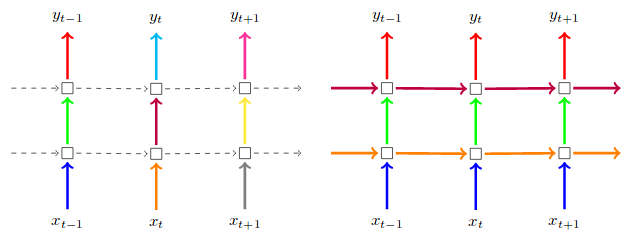
\includegraphics[scale=0.4]{recurrent_drop_out_rate.png}
Here the regular drop out drops the connection to or from input/output layers (i.e. vertical arrows) whereas the recurrent drop out drops the connections between hidden layers (the horizontal arrows). In our case it performed the best at 0.2.
%https://arxiv.org/pdf/1512.05287.pdf
\\ \emph{Patience for Early Stopping}
\par Early stopping is a regularization process where the possibility of overfitting is reduced by the following procedure.
The first step is to keep track of training and validation accuracy - or any other evaluation metric of choice - at each epoch. Then at the end of each epoch remark how the metric for the validation set changes; if it continuously decreases for a certain number of epoch, the learning process gets terminated early (hence the procedure is named so). The hyperparameter for this procedure would be the number of epoch to observe the decreasing trend of validation metric (or how many epochs we would "allow" to continue even if the validation metric decreases), or commonly known as the patience. Something to remark for our model is that as the magnitude of patience increases the model performed more poorly on the validation set for both the restaurant dataset and data for laptop reviews. Our hyperparameter tuning showed the models performed the best at patience of 2.
\\ \emph{Choice of activation function:}
For any neural network the choice of activation function, particularly for hidden layers is crucial. The list of choices available to us to Rectified linear units, tanh, and sigmoid functions. After tuning we concluded that having ReLu function for hidden layers and sigmoid for the output layers give the best models.
%-What loss function was used to analyze the models
\par For LSTM and GRU, the loss function used to evaluate the performance is categorical cross entropy supported from keras library. I.e. the loss function $J(\vec{w})$ would be
\[
J(\vec{\theta}) = - \sum_{n=1}^N\sum_{m=1}^M\{1\{y^{(n)}=k\}\log P(y^{(i)} = k|x^{(i)}; \theta)\}
\]

which is a multinomial generalization of the binary case
\[
J(\vec{w})- \frac{1}{N} [ \sum_{n=1}^N \{y^{(n)} \log \hat{y}^{(n)}(\vec{x}) + (1-y^{(i)})\log(1-\hat{y}^{(n)}(\vec{x})) \}]
\]
where $\hat{y}(\vec(x)) = \frac{1}{1+e^{\vec{w}^t\vec{x}}}$

In order to avoid overfitting, we have adopted early stopping with patience level of 2-16 as our regularization method. Another choice of ours is regular dropout with rate 0.5 with recurrent drop out with rate 0.2. The method of early stopping prevents overfitting in the sense that it stops the entire learning procedure once it starts learning the "unnecessary" traits from the training set, making sure that it will not go through situations where the model would overfit. Both of the drop out methods check the existence of a particular unit or neuron that has picked up the features/traits that are specific to the training set.

% Evaluation metric
We have identified the various sentiment categories as positive, negative, and neutral. The result is compared with the standard annotations provided in the dataset and the accuracy is computed as
$$
\textbf{accuracy} = \frac{\textbf{TP}+\textbf{TN}}{\textbf{TP}+\textbf{FP}+\textbf{FN}+\textbf{TN}}
$$

\begin{table*}
\label{my-label}
\begin{tabularx}{\textwidth}{@{}l*{11}{C}c@{}}
\toprule
Domain (Representation) & CNN (paper) & LSTM (paper) & LSTM & GRU & Naive Bayes & Logistic Reg. & Linear SVM & Radial SVM & Decision Trees & Random Forest \\ 
\midrule
Restaurants (GloVe)    & 82.10 & 81.40 & \textbf{90.76} & 88.57 & -     & -     & -     & -     & -     & -     \\
Restaurants (BBoW)     & -     & -     & -              & -     & 79.88 & 79.59 & 80.03 & 72.89 & 73.62 & 77.26 \\
Restaurants (FBoW)     & -     & -     & -              & -     & 80.76 & 80.47 & 78.72 & 72.45 & 72.89 & 78.57 \\
Restaurants (TFIDF)    & -     & -     & -              & -     & 83.24 & 81.92 & 82.51 & 73.47 & 73.76 & 77.55 \\
Laptops (GloVe)        & 78.40 & 76.00 & \textbf{87.93} & 85.50 & -     & -     & -     & -     & -     & -     \\
Laptops (BBoW)         & -     & -     & -              & -     & 69.50 & 70.82 & 68.70 & 56.76 & 66.31 & 69.23 \\
Laptops (FBoW)         & -     & -     & -              & -     & 71.75 & 69.23 & 68.70 & 40.98 & 62.33 & 68.70 \\
Laptops (TFIDF)        & -     & -     & -              & -     & 73.87 & 69.23 & 72.68 & 57.29 & 61.14 & 65.52 \\
\bottomrule
\end{tabularx}
\caption{Summary of results for each classifier, where the evaluation metric is accuracy (4 s.f.) and highest scores are bolded}
\end{table*}

\section{Results}
%Summary: table of results (accuracy metric), graphs (hyper-parameters, loss vs. epochs, etc), compare models, compare datasets (rest vs. lapt), compare hyper-parameters, note an example which algorithms analyze a sentence difference (if possible), note what features of a model appears to bring up/down the performance
To represent the aspect given as our input, we have encoded our aspect as a binary vector v $\in \mathbb{F}_2 ^n$ where n=12 for the restaurant data, and n=15 for the laptop data. Then we concatenate this aspect vector to the original Bag-of-word representation. Overall this concatenation, when compared to naive sentiment analysis without aspect taken as input, generally underfit for the training yet demonstrates an improved level of performance for both the validation and test set.

We disregard the extremely randomized tree classifiers since it is computationally expensive (it takes more than an hour to train one tree) and severly underfits.

We add the support vector machine classifier with a non linear kernel(for this case it is namely the radial basis function) to see whether this would bring a model with better performance.

The results suggest that provided the concatenated input features, the linear support vector machine models performs extremely well, even to the point where it surpasses the evaluation metric of one of the baselines (namely LSTM). It is also something to remark that the random forest classifier shows a decent fit.

\par Further additional preprocessing measures such as trimming words or lemmatization seems to penalize against the models where aspects are not taken as input, but one can remark that it actually helps those where aspects are taken as features. This is a better result for us since our main focus here is to show the importance of Aspect-Based sentimental analysis. However, one can conclude that this might be heavily dependent on the number of aspects one is given as input for a model. This will be discussed further and in details in Section VI.

The SVM with the non linear kernel surprisingly underperforms compared to its linear equivalent, suggesting the dataset might be linearly separable.
\par Something to remark from the neural network models (LSTM and GRU) is that the accuracy we have obtained from the models do far better than the results on the original work. Graph A is the crossentropy vs epoch graph from GRU model with 45 hidden layer units for the restaurant dataset. We can remark that there is slight tendency of overfitting at the end of the 10th epoch, when the learning procedure stopped early due to early stopping regularization. Graph B  is a graph of learning procedure description for the laptop dataset. We can see overall it shows a worse fit than the model on the restraurant reviews. Graph C and D show the respective learning procedure for the both LSTM models with 45 hidden units. It shows a far stable and a better fit compared to the previous GRU models.

\newpage
\begin{figure}[hp]
\centering
\textbf{Graph A }\par\medskip
\caption{GRU Model on restaurant dataset with 45 number of hidden layers}
\includegraphics[scale=0.4]{hl45rest.png}
\end{figure}
\begin{figure}[hp]
\centering
\textbf{Graph B}|\par \medskip 
\caption{GRU Model on laptop dataset with 45 number of hidden layers}
\includegraphics[scale=0.4]{hl45lapt.png}
\end{figure}

\begin{figure}[hp]
\centerin
\textbf{Graph C} \par \medskip 
\caption{LSTM Model on restaurant dataset with 45 number of hidden layers}
\includegraphics[scale=0.4]{hl45LSTM.png}
\end{figure}




\newpage
\begin{figure}[hp]
\centerin
\textbf{Graph D} \par \medskip 
\caption{LSTM Model on laptop dataset with 45 number of hidden layers}
\includegraphics[scale=0.4]{hl45LSTMlapt.png}
\end{figure}

\newpage
\section{Discussion:}

%-Computational time for Random Forest and LSTM
\par One can remark that using pre-trained word embeddings (namely GloVe for the case of interest) results in a significant gain in terms of efficiency. However, when we restrict our focus on the context where the number of aspects in input is small, bag-of-words representation could still present a decently well constructed model. 
\par One concern is that we might need to depend on neural networks or a more recently developed model in case where one needs to do Aspect-Based sentimental analysis with an asymptotic number of possible aspects that a model needs to recognize. In all of the results we have obtained we could remark that for the laptop reviews (where the number of aspects were close to 100) all of the classical model demonstrate a relatively poor fit. This does not change even when we group of some of the aspects with relatively fewer occurences as $\texttt{OTHER}$. 
\par Out of the classical ML algorithms, there are three types of classifiers to remark: Multinomial Naive Bayes, Random Forests, and Linear SVM classifiers.
\\\emph{Multinomial Naive Bayes}
\par Multinomial Naive Bayes shows a huge improvement in performance since the additional preprocessing measure. The test accuracy shows more than 10 percent increase once the lemmatization applies. One question that might arise is the level of performance improvement is less pronounced for Bernoulli Naive Bayes model is mostly binary (there are a few entries with polarity "neutral" yet most of them are either "positive" or "negative".) It seems that the conditional independence assumption of response given the features describe our dataset well enough. It also outperformed the baselines if tf-idf representation is used instead of mere bag-of-words.
\\ \emph{Random Forests}
\par Preprocessing makes another classifier to be one of the top candidates to beat the baselines among the classical ML algorithms. Random forests show a particularly show a greatly overfitting results for the laptop review dataset, staying consistent in what we have learned from classnotes that decision tree and random forests tend to overfit when the number of feature needed to learn increases.
\\ \emph{Linear SVM}
\par Linear SVM under the bag-of-words  representation with preprocessed sentences is, indeed, one of the classifiers with the best performance. On restaurant review datasets, it outperforms the performance of LSTM in the reference paper
\\ \emph{Logistic Regression}
\par Logistic models have been our strong candidate as classical ML algorithms to outperform the results in the reference paper since it works well on sparse matrices, which are common in sentiment analysis problems. Under tf-idf vectorization the logistic classifier performed on par with linear SVM.  Which is a really a remarkable point.
\par However, it seems that as the number of aspects increase asymptotically the fit significantly gets worse. For laptop review data sets all the models show at least ten percent decrease in accuracy.
Unlike the models with a non linear kernels ( e.g. cubic polynomial or the radial basis function) linear SVM performs a consistent fit as well, suggesting the data might be linearly separable.
\par Out of the neural networks we have fit, namely two models: Gated recurrent units and Long   short term memory units. Even though both networks are known for demonstrating a great performance on sentiment analysis and natural language processing, in our case LSTM did far better. One possible reason for is that LSTM networks are capable for remembering longer sequences of words than GRUs (GRUs delete some piece of information from the past using reset gates)
\par The early stopping procedure really helps in terms of saving the duration time for the learning procedure. The training procedure for all the neural network models supposedly has 1000 epochs, yet most of them terminate in the midst of the learning as soon as they overfit. While not using an virtual instance from a cloud computing service, all the neural network training procedures took less than 10 minutes
\par Changing the dropout rate did not really contribute much, surprisingly. One thing our team conjectures is that the effect of dropout might be significant once the training process gets long enough, where it never gets to happen in our case due to the early stopping
\par As we can see from the graphs above most of our model show a very good learning procedure curve (no significant sign of overfitting or underfitting).
\section{Conclusion}
\par The hypothesis raised in our team's proposal that some classical ML algorithms that perform well on sparse matrices such as logistic regression seems to have some evidence. Something to remark is the surprisingly good performance of Multinomial naive Bayes models.
\par Out of the neural network models the LSTM shows the best fit for both of the datasets, possibly due to the nature of the reviews where long term dependencies are common. It shows why LSTM is clearly one of the top choices for tasks in natural language processing and in particular sentiment analysis. GRU models, on the other hand, have been implemented in a very time efficient manner, yet it clearly shows a worse fit. To conclude, one should distinguish with care the context when  to choose which  of two neural network models.

\section{Contribution} 
The authors, Ramsha Ijaz, Aanika Rahman and Dan Yunheum Seol, have all taken direct roles in all classifier implementations, methodology and model evaluations, feature preprocessing, as well as the composition of the report. 

We hereby state that all the work presented in this report is that of the authors.

\newpage \no
\section*{Appendix}

\begin{figure}[!htbp]
\centering
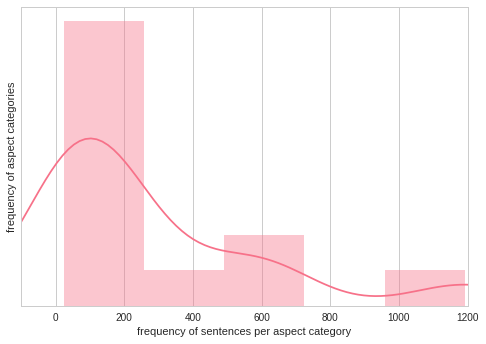
\includegraphics[scale=0.5]{images/anal_asp-freq_REST.png}
\caption{Distribution of aspect categories (REST)}
\end{figure}
\begin{figure}[!htbp]
\centering
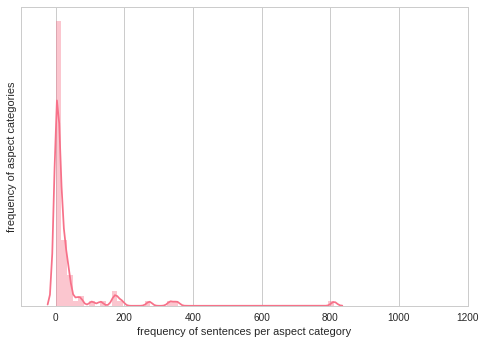
\includegraphics[scale=0.5]{images/anal_asp-freq_LAPT.png}
\caption{Distribution of aspect categories (LAPT)}
\end{figure}

\bibliographystyle{plain}
\bibliography{report}

\end{document}